\let\lesson\undefined
\newcommand{\lesson}{\phantomlesson{Bài 12: Một số lực trong thực tiễn}}
\chapter[Trọng lực và lực căng]{Trọng lực và lực căng}
\setcounter{section}{0}
\section{Lý thuyết}
\subsection{Trọng lực - Lực hấp dẫn}
\subsubsection{Lực hấp dẫn}
Mọi vật trong vũ trụ đều hút nhau với một lực, gọi là lực hấp dẫn.

Đặc điểm của lực hấp dẫn:	
\begin{itemize}
	\item Luôn là lực hút;
	\item Là lực không tiếp xúc (tác dụng từ xa).
\end{itemize}

\subsubsection{Định luật vạn vật hấp dẫn} 
\begin{center}
	\begin{tikzpicture}
		\coordinate (A1) at (0,0);
		\coordinate (A2) at ($(A1)+(1.5cm,0)$);
		\coordinate (B1) at ($(A1)+(6cm,0)$);
		\coordinate (B2) at ($(B1)-(1.5cm,0)$);
		\shade[ball color=green] (A1) circle (0.75cm); 
		\shade[ball color=purple] (B1) circle (0.5cm);
		\draw[dashed] (A1) -- (B1);
		\draw[->,very thick] (A1)--(A2) node[near end,above right]{$\vec{F}_{12}$};
		\draw[->,very thick] (B1)--(B2) node[near end,above left]{$\vec{F}_{21}$};
		\coordinate (Ad) at ($(A1)-(0,2cm)$);
		\coordinate (Bd) at ($(B1)-(0,2cm)$);
		\draw[dotted] (A1) -- (Ad);
		\draw[dotted] (B1) -- (Bd);
		\draw[<->] (Ad) --(Bd);
		\node[below=1cm, fill=pagecol] at (A1) {$m_1$};
		\node[below=0.75cm, fill=pagecol] at (B1) {$m_2$};
		\node[fill=pagecol] at ($(Ad)!0.5!(Bd)$) {$r$};
	\end{tikzpicture}
\end{center}
Lực hấp dẫn giữa hai chất điểm bất kì tỉ lệ thuận với tích hai khối lượng của chúng và tỉ lệ nghịch với bình phương khoảng cách giữa chúng.
\begin{equation*}
	F_{\text {hd}} = G \dfrac {m_1 m_2 }{r^2},
\end{equation*}
trong đó:
\begin{itemize}
	\item $G$ là hằng số hấp dẫn, trong hệ SI có giá trị $G=\SI{6.67e-11}{\newton \meter ^2/\kilogram ^2}$;
	\item $m_1$, $m_2$ là khối lượng của hai vật;
	\item $r$ là khoảng cách giữa hai vật.
\end{itemize}

\subsubsection{Trọng lực }

Trọng lực là lực hấp dẫn của Trái Đất tác dụng vào vật gây ra cho chúng gia tốc rơi tự do. Trọng lực kí hiệu là $\vec P.$\\
Độ lớn của trọng lực:
\begin{equation*}
	P=F_{\text{hd}}=G \dfrac {mM}{(R+h)^2},
\end{equation*}
trong đó:
\begin{itemize}
	\item $m$ là khối lượng của vật ($\SI{}{\kilogram}$);
	\item $M$ là khối lượng Trái đất ($M \approx \SI{6e24}{\kilogram}$);
	\item $R$ là bán kính Trái đất ($R \approx \SI{6400e3}{\meter}$);
	\item $h$ là  độ cao của vật so với mặt đất ($\SI{}{\meter}$).
\end{itemize}

Gia tốc rơi tự do:
\begin{equation*}
	g=G \dfrac {M}{(R+h)^2}.
\end{equation*}
\begin{center}
	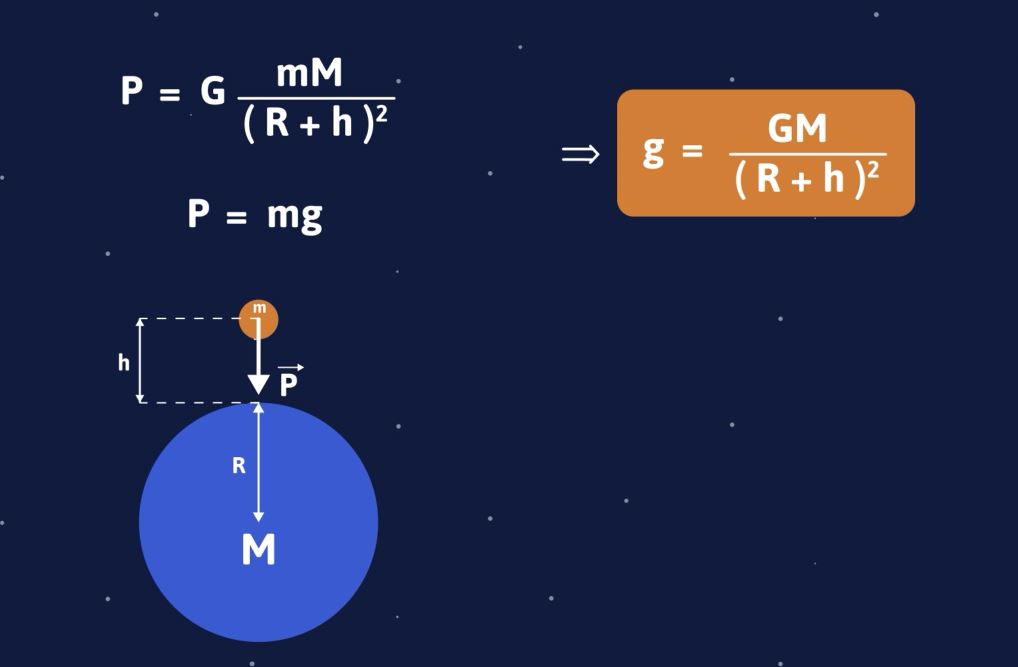
\includegraphics[scale=0.4]{../figs/VN10-PH-13-A-004-1-V2-01.jpg}
\end{center}
Ở gần Trái đất, trọng lực có phương thẳng đứng, có chiều từ trên xuống. \\
Công thức tính trọng lực: 
\begin{equation*}
	\vec P=m\vec g.
\end{equation*}

\subsubsection{Trọng lượng}
Khi vật đặt trong trọng trường và ở trạng thái cân bằng nhờ một dây treo hay giá đỡ, thì độ lớn của lực căng dây hoặc lực ép của vật lên giá đỡ gọi là trọng lượng của vật.  

\luuy{Không nên nhầm lẫn rằng trọng lượng là độ lớn của trọng lực. 
	
	Ví dụ, phi hành gia trên các trạm vũ trụ vẫn chịu tác dụng của trọng lực $P=mg$. Tuy nhiên nếu đặt một cái cân dưới chân phi hành gia thì cân chỉ số 0, vì trọng lực đã cân bằng với lực quán tính ly tâm (do trạm vũ trụ quay quanh Trái đất), nên phi hành gia không tạo được sức ép vào mặt cân. Ta nói phi hành gia ở trạng thái không trọng lượng (chứ không phải không trọng lực).}
\subsection{Lực căng dây}
\begin{minipage}[l]{0.5\textwidth}
	Khi kéo căng một sợi dây thì trong sợi dây xuất hiện lực căng chống lại xu hướng bị kéo dãn, gọi là lực căng dây. Lực căng dây kí hiệu là $\vec{T}$.

	Đối với dây không co giãn và khối lượng không đáng kể, độ lớn lực căng dây là như nhau tại mọi điểm trên dây. 
	
\end{minipage}
\begin{minipage}[r]{0.5\textwidth}
	\begin{center}
		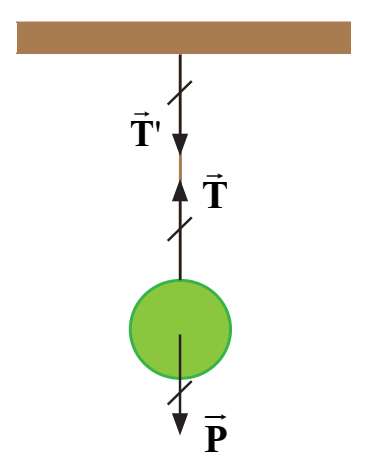
\includegraphics[width=0.3\linewidth]{../figs/VN10-2023-PH-TP018-1}
		\captionof{figure}{Qủa cầu ở trạng thái cân bằng.}
	\end{center}
\end{minipage}
\section{Mục tiêu bài học - Ví dụ minh họa}
\begin{dang}{Ghi nhớ định luật vạn vật hấp dẫn. \\Nhận biết được đặc điểm của lực hấp dẫn}
	\viduii{1}{Lực hấp dẫn do một hòn đá ở trên mặt đất tác dụng vào Trái Đất thì có độ lớn
		\begin{mcq}(2)
			\item lớn hơn trọng lực của hòn đá.
			\item nhỏ hơn trọng lực của hòn đá.
			\item bằng trọng lực của hòn đá. 
			\item bằng 0.
		\end{mcq}
	}
	{\hide{
		Theo định luật III Newton: lực hấp dẫn do Trái Đất tác dụng lên hòn đá bằng lực hấp dẫn do hòn đá tác dụng lên Trái Đất.
		
		\textbf{Đáp án: C.}
	}}

	\viduii{1}{Chọn phát biểu sai về lực hấp dẫn giữa hai vật?
		\begin{mcq}
			\item Lực hấp dẫn tăng 4 lần khi khoảng cách giảm đi một nửa .
			\item Lực hấp dẫn không đổi khi khối lượng một vật tăng gấp đôi còn khối lượng vật kia giảm còn một nửa.
			\item Rất hiếm khi lực hấp dẫn là lực đẩy.
			\item Hằng số hấp dẫn có giá trị như nhau ở cả trên mặt Trái Đất và trên Mặt Trăng.
		\end{mcq}
		
	}
	{\hide{
		Lực hấp dẫn luôn là lực hút.
		
		\textbf{Đáp án: C.}
	}}
\end{dang}

\begin{dang}{Tính lực hấp dẫn và các đại lượng trong công thức của định luật vạn vật hấp dẫn}
	\viduii{3}{Cho biết khoảng cách giữa tâm Mặt Trăng và tâm Trái Đất là $\SI{38e7}{\meter}$; khối lượng Mặt Trăng và Trái Đất tương ứng là $\SI{7.37e22}{\kilogram}$ và $\SI{6e24}{\kilogram}$; hằng số hấp dẫn $G = \SI{6.67e-11}{\newton \meter ^2 / \kilogram ^2}$. Lực hấp dẫn giữa Trái Đất và Mặt Trăng có độ lớn là
		\begin{mcq}(2)
			\item $\SI{0.204e21}{\newton}$.
			\item $\SI{2.04e21}{\newton}$.
			\item $\SI{22e2}{\newton}$.
			\item $\SI{2e27}{\newton}$.
		\end{mcq}
	}
	{\hide{
		Áp dụng công thức lực hấp dẫn giữa Trái Đất và Mặt Trăng
		$$	F_{\text{hd}}=G\dfrac {m_1 m_2}{r^2} = \SI{0.204e21}{\newton}.$$
		
		\textbf{Đáp án: A.}
		
	}}

	\viduii{3}{Hai quả cầu giống nhau được đặt sao cho hai tâm cách nhau khoảng $r$ thì lực hấp dẫn giữa chúng là $F$. Nếu thay một trong hai khối cầu trên bằng một khối cầu đồng chất khác nhưng có bán kính lớn gấp hai, vẫn giữ nguyên khoảng cách giữa hai tâm (hai khối cầu không chạm nhau) thì lực hấp dẫn giữa chúng lúc này là
		\begin{mcq}(4)
			\item $2F$.
			\item $4F$.
			\item $8F$.
			\item $16F$.
		\end{mcq}
		
	}
	{\hide{
		Gọi quả cầu 2 là quả cầu có bán kính tăng gấp đôi. Bán kính của quả cầu 2 lúc sau
		$$r_2 ' = 2 r_2.$$
		
		Nếu $D$ là khối lượng riêng của quả cầu thì khối lượng của quả cầu 2 lúc sau sẽ là 
		$$m_2 ' = D V_2 ' = D\cdot \dfrac{4}{3}\pi {r'}_2^3= D\cdot \dfrac {4}{3} \pi (2r_2) ^3 = 8 D\cdot \dfrac {4}{3}\pi r_2 ^3 = 8 D V_2 = 8 m_2. $$
		
		Lực hấp dẫn giữa hai quả cầu lúc sau
		$$F_\text{hd}' = G \dfrac{m_1 m_2 '}{r^2} = 8 G \dfrac {m_1 m_2}{r^2} = 8F.$$
		
		\textbf{Đáp án: C.}
	}}
\end{dang}
\begin{dang}{Tính gia tốc rơi tự do và  trọng lượng vật trong các điều kiện khác nhau}
	\viduii{3}{Ở độ cao nào so với mặt đất thì gia tốc rơi tự do bằng một nửa gia tốc rơi tự do ở mặt đất? Cho bán kính Trái Đất là $R=\SI{6400}{\kilo \meter}$.
	}
	{\hide{
		Gia tốc rơi tự do ở mặt đất:
		$$g_0 = G \dfrac {M}{R^2}.$$
		
		Gia tốc rơi tự do ở độ cao $h$:
		$$g=G \dfrac {M}{(R+h)^2}.$$
		
		Gia tốc rơi tự do ở độ cao $h$ bằng một nửa gia tốc rơi tự do ở mặt đất, nên
		$$g=\dfrac{g_0}{2} \Rightarrow G \dfrac {M}{(R+h)^2} = G \dfrac {M}{2R^2} \Rightarrow (R+h)^2 = 2 R^2 \Rightarrow h=\SI{2650}{\kilo \meter}.$$
		
		Vậy ở độ cao $h=\SI{2650}{\kilo \meter}$ so với mặt đất thì gia tốc rơi tự do bằng một nửa so với gia tốc rơi tự do ở mặt đất.
		
	}}

	\viduii{3}{Tính độ cao mà ở đó gia tốc rơi tự do là 9,6 m/s$^2$. Biết bán kính Trái Đất là 6400 km và gia tốc rơi tự do ở sát mặt đất là 9,8 m/s$^2$.
	}
	{\hide{
		Gia tốc rơi tự do ở độ cao $h$ 
		\begin{equation*}
			g = \dfrac{GM}{(R+h)^2} = \text{9,6}\ \text{m/s}^2.
		\end{equation*}
		Gia tốc rơi tự do ở sát mặt đất 
		\begin{equation*}
			g_0 = \dfrac{GM}{R^2} = \text{9,8}\ \text{m/s}^2.
		\end{equation*}
		Suy ra 
		\begin{equation*}
			\dfrac{g}{g_0}= \left(\dfrac{R}{R+h}\right)^2 =\text{0,98}\Rightarrow h = \dfrac{R(1- \sqrt{\text{0,98}})}{\sqrt {\text{0,98}}} = 65\ \text{km}.
		\end{equation*}
		
	}}
\end{dang}
\begin{dang}{Mô tả được bằng ví dụ thực tiễn và biểu diễn được bằng hình vẽ: trọng lực, lực căng dây}
	\viduii{2}
	{Một bóng đèn có khối lượng $\SI{500}{\gram}$ được treo thẳng đứng vào trần nhà bằng một sợi dây và đang ở trạng thái cân bằng.
		\begin{enumerate}[label=\alph*)]
			\item Biểu diễn các lực tác dụng lên bóng đèn.
			\item Tính độ lớn của lực căng dây.
			\item Nếu dây treo chỉ chịu được một lực căng giới hạn $\SI{5.5}{\newton}$ thì nó có bị đứt không?
		\end{enumerate}
}
{\hide{
\begin{enumerate}[label=\alph*)]
\begin{minipage}[l]{0.6\textwidth}
\item Các lực tác dụng lên bóng đèn gồm:
	\begin{itemize}
		\item Trọng lực phương thẳng đứng hướng xuống.
		\item Lực căng dây phương thẳng đứng hướng lên.
	\end{itemize}
\item Vì bóng đèn đang ở trạng thái cân bằng nên:
$$T=P=mg=\left(\SI{0.5}{\kilogram}\right)\cdot\left(\SI{9.8}{\meter/\second^2}\right)=\SI{4.9}{\newton}$$
\item Dây không bị đứt vì lực căng mà dây phải chịu là $\SI{4.9}{\newton}$ nhỏ hơn lực căng giới hạn.
\end{minipage}
\begin{minipage}{0.4\textwidth}
	\begin{center}
		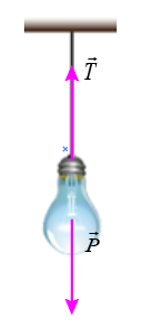
\includegraphics[width=0.3\linewidth]{../figs/VN10-2023-PH-TP018-2}
	\end{center}
\end{minipage}
\end{enumerate}
}}
\end{dang}
\begin{dang}{Tính các lực tác dụng lên vật \\khi vật cân bằng}
	\viduii{3}{Một vật có trọng lượng $P= 10$ N. được treo vào một vòng nhẫn O (coi là chất điểm). Vòng nhẫn được giữ yên bằng hai dây OA và OB. Biết dây OA nằm ngang và hợp với dây OB một góc $120^\circ.$ Tìm lực căng dây của hai dây OA và OB.
		
		\begin{center}
			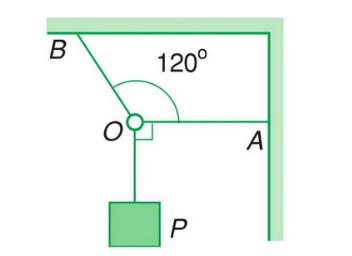
\includegraphics[scale=0.5]{../figs/VN10-PH-11-L-008-4-V2-01.jpg}
		\end{center}
	}
	{\hide{
		\textbf{Cách 1: Áp dụng quy tắc tổng hợp lực.}
		\begin{center}
			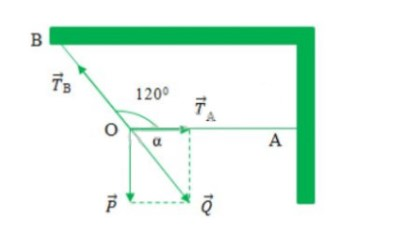
\includegraphics[scale=0.8]{../figs/VN10-PH-11-L-008-4-V2-02.jpg}
		\end{center}
		Khi vật ở vị trí cân bằng thì các lực tác dụng lên vật gồm trọng lực $\vec{P}$, lực căng trên hai dây $\vec{T}_A$ và $\vec{T}_B$. Vòng nhẫn đứng yên nên các lực cân bằng nhau
		$$\vec{P}+\vec{T}_\textrm{A}+\vec{T}_\textrm{B}=\vec{0}.$$
		Gọi $\vec{Q}$ là hợp lực của $\vec{P}$ và $\vec{T}_A$
		$$\vec{P}+\vec{T}_\textrm{A}=\vec{Q}\quad\Rightarrow \quad\vec{T}_\textrm{B}+\vec{Q}=\vec{0}\quad\Rightarrow\quad \vec{T}_\textrm{B}=-\vec{Q}$$
		nghĩa là $\vec{Q}$ và $\vec{T}_B$ là hai vector trực đối. Do đó, $\alpha =\SI{	180}{\degree}-\SI{120}{\degree}=\SI{60}{\degree}.$
		
		Xét $\triangle$O$T_\text{A}$Q vuông tại $T_\text{A}$:
		
		$$\tan \alpha =\dfrac{P}{T_\text{A}}\Rightarrow T_\text{A}=\dfrac{P}{\tan \alpha}=\dfrac{10\sqrt{3}}{3}\,\text{N}.$$
		$$\sin \alpha =\dfrac{P}{Q}\Rightarrow Q=\dfrac{P}{\sin \alpha}=\dfrac{20\sqrt{3}}{3}\,\text{N}.$$
		Vì $|\vec{T}_\textrm{B}|=|\vec{Q}|$ nên $T_\textrm{B}= \dfrac{20\sqrt{3}}{3}\,\text{N}.$
		
		Vậy lực căng dây của hai dây OA và OB lần lượt bằng $\dfrac{10\sqrt{3}}{3}\,\text{N}, \dfrac{20\sqrt{3}}{3}\,\text{N}.$\\
		\textbf{Cách 2: Áp dụng quy tắc tam giác lực}\\
		Vòng nhẫn đứng yên nên các lực cân bằng nhau
		$$\vec{P}+\vec{T}_\textrm{A}+\vec{T}_\textrm{B}=\vec{0}.$$
		Do đó, $\left(\vec{P}, \overrightarrow{T_A}, \overrightarrow{T_B}\right)$ tạo thành tam giác khép kín
		\begin{center}
			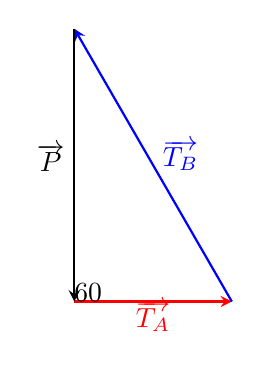
\begin{tikzpicture}
				\coordinate (O) at (2,0);
				\coordinate (A) at (0,0);
				\coordinate (B) at (0,3.464);
				\coordinate (O1) at (1,0);
				\coordinate (A1) at (1,1.73);
				\coordinate (B1) at (0,1.7);
				\draw[-stealth,thick, red] (A) -- (O);
				\draw[-stealth,thick, blue] (O) -- (B);
				\draw[-stealth,thick] (B) -- (A);
				\node[label={[red,below]90:$\overrightarrow{T_A}$}] at (O1){};	
				\node[label={[blue,right]90:$\overrightarrow{T_B}$}] at (A1){};	
				\node[label={[black,left]90:$\overrightarrow{P}$}] at (B1){};	
				\tkzMarkAngle[size=0.4,color=black](B,O,A);
				\tkzLabelAngle[color=black,pos=0.8](B,O,A){$\SI{60}{\degree}$}
				\tkzMarkRightAngle[draw=black,size=.25](B,A,O);
			\end{tikzpicture}
		\end{center}
		Từ tam giác vectơ ta xác định được 
		\begin{align*}
			\begin{cases}
				T_A=\dfrac{P}{\tan\SI{60}{\degree}}=\xsi{\dfrac{10\sqrt{3}}{3}}{\newton}\\
				T_B=\dfrac{P}{\sin\SI{60}{\degree}}=\xsi{\dfrac{20\sqrt{3}}{3}}{\newton}
			\end{cases}
		\end{align*}
		
	}}

	\viduii{3}{Một đèn tín hiệu giao thông ở đại lộ có trọng 
		lượng 120 N được treo vào trung điểm của dây 
		AB làm dây thòng xuống $\text{0,5}$ m. Cho biết hai trụ treo dây cách nhau \SI{8}{\meter}, bỏ qua 
		trọng lượng của dây, tính lực căng mỗi sợi dây. 
		\begin{center}
			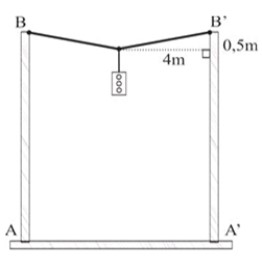
\includegraphics[scale=0.7]{../figs/VN10-PH-11-L-008-4-V2-03.jpg}
		\end{center}
	}
	{\hide{
		\textbf{Cách 1: Phân tích lực.}
		\begin{center}
			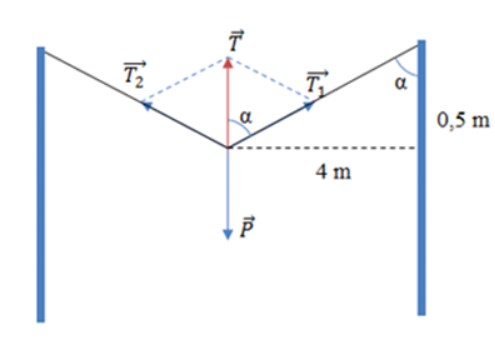
\includegraphics[scale=0.5]{../figs/VN10-PH-11-L-008-4-V2-04.jpg}
		\end{center}
		Đèn khi cân bằng chịu các lực tác dụng như hình vẽ, gồm trọng lực $\vec{P}$, hai lực căng dây $\vec{T}_1$ và $\vec{T}_2$
		\begin{align*}
			\vec{P}+\vec{T}_1+\vec{T}_2=0
		\end{align*}
		
		Gọi $\vec T$ là hợp lực của hai dây cáp:
		$$\vec{T}=\vec{T}_1+\vec{T}_2\quad\Rightarrow\quad \vec{P}+\vec{T}=0$$
		nghĩa là $T=P=mg=\SI{120}{\newton}$.
		
		Do tính đối xứng, hai lực căng dây phải có độ lớn bằng nhau $T_1=T_2$. Từ hình vẽ 
		\begin{align*}
			T=2T_1\cos \alpha\quad\Rightarrow\quad T_1=\dfrac{T}{2\cos\alpha}
		\end{align*}
		trong đó góc $\alpha$ được xác định từ tam giác vuông bên phải trên hình
		\begin{align*}
			\tan\alpha=\dfrac{\SI{4}{\meter}}{\SI{0.5}{\meter}}=8\quad\Rightarrow\quad \alpha\approx\SI{82.875}{\degree}. 
		\end{align*}
		Từ đó ta tính được lực căng dây
		\begin{align*}
			T_1=T_2=\dfrac{T}{2\cos\alpha}\approx \SI{484}{\newton}.
		\end{align*}		
	\textbf{Cách 2: Dùng tam giác lực}\\
	Đèn cân bằng nên
	\begin{align*}
		\vec{P}+\vec{T}_1+\vec{T}_2=\overrightarrow{0}
	\end{align*}
Do tính đối xứng, hai lực căng dây phải có độ lớn bằng nhau $T_1=T_2$.\\
Ba vectơ lực $\vec{P}, \overrightarrow{T_1}, \overrightarrow{T_2}$ tạo thành tam giác vectơ khép kín
	\begin{center}
	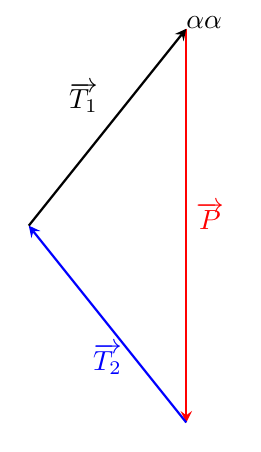
\begin{tikzpicture}
		\coordinate (O) at (0,0);
		\coordinate (A) at (0,-5);
		\coordinate (B) at (-2,-2.5);
		\coordinate (O1) at (0,-2.5);
		\coordinate (A1) at (-1,-4);
		\coordinate (B1) at (-1,-1);
		\draw[-stealth,thick, red] (O) -- (A);
		\draw[-stealth,thick, blue] (A) -- (B);
		\draw[-stealth,thick] (B) -- (O);
		\node[label={[red,right]90:$\overrightarrow{P}$}] at (O1){};	
		\node[label={[blue,below]90:$\overrightarrow{T_2}$}] at (A1){};	
		\node[label={[black,left]90:$\overrightarrow{T_1}$}] at (B1){};	
		\tkzMarkAngle[size=0.5,color=black](O,A,B);
		\tkzLabelAngle[color=black,pos=0.8](O,A,B){$\alpha$};
		\tkzMarkAngle[size=0.5,color=black](B,O,A);
		\tkzLabelAngle[color=black,pos=0.8](B,O,A){$\alpha$}
	\end{tikzpicture}
\end{center}
Áp dụng định lý hàm sin:
\begin{align*}
	\dfrac{T_1}{\sin\alpha}&=\dfrac{P}{\sin\left(\SI{180}{\degree}-2\alpha\right)}\Leftrightarrow \dfrac{T_1}{\sin\alpha}=\dfrac{P}{\sin\left[2\cdot\left(\SI{90}{\degree}-\alpha\right)\right]}\\
	\Rightarrow \dfrac{T_1}{\sin\alpha}&=\dfrac{P}{2\sin\left(\SI{90}{\degree}-\alpha\right)\cos\left(\SI{90}{\degree}-\alpha\right)}=\dfrac{P}{2\cos\alpha\sin\alpha}\\
	\Rightarrow T_1&=\dfrac{P}{2\cos\alpha}\approx\SI{484}{\newton}
\end{align*}
	}}
	
	
\end{dang}